%% LyX 2.2.1 created this file.  For more info, see http://www.lyx.org/.
%% Do not edit unless you really know what you are doing.
\documentclass[twocolumn,conference]{IEEEtran}
\usepackage[LGR,T1]{fontenc}
\usepackage[latin9]{inputenc}
\usepackage{refstyle}
\usepackage{booktabs}
\usepackage{textcomp}
\usepackage{graphicx}
\usepackage[unicode=true,
 bookmarks=true,bookmarksnumbered=true,bookmarksopen=true,bookmarksopenlevel=1,
 breaklinks=false,pdfborder={0 0 0},pdfborderstyle={},backref=false,colorlinks=false]
 {hyperref}
\hypersetup{
 pdfauthor={Ahmad Abdullah},
 pdfpagelayout=OneColumn, pdfnewwindow=true, pdfstartview=XYZ, plainpages=false}
\usepackage{breakurl}

\makeatletter

%%%%%%%%%%%%%%%%%%%%%%%%%%%%%% LyX specific LaTeX commands.

\AtBeginDocument{\providecommand\secref[1]{\ref{sec:#1}}}
\AtBeginDocument{\providecommand\figref[1]{\ref{fig:#1}}}
\AtBeginDocument{\providecommand\subsecref[1]{\ref{subsec:#1}}}
\AtBeginDocument{\providecommand\tabref[1]{\ref{tab:#1}}}
\DeclareRobustCommand{\greektext}{%
  \fontencoding{LGR}\selectfont\def\encodingdefault{LGR}}
\DeclareRobustCommand{\textgreek}[1]{\leavevmode{\greektext #1}}
\ProvideTextCommand{\~}{LGR}[1]{\char126#1}

%% Because html converters don't know tabularnewline
\providecommand{\tabularnewline}{\\}
\RS@ifundefined{subsecref}
  {\newref{subsec}{name = \RSsectxt}}
  {}
\RS@ifundefined{thmref}
  {\def\RSthmtxt{theorem~}\newref{thm}{name = \RSthmtxt}}
  {}
\RS@ifundefined{lemref}
  {\def\RSlemtxt{lemma~}\newref{lem}{name = \RSlemtxt}}
  {}


%%%%%%%%%%%%%%%%%%%%%%%%%%%%%% User specified LaTeX commands.
% for subfigures/subtables
\usepackage[caption=false,font=footnotesize]{subfig}
%\newref{fig}{name = \RSFigtxt}
%\newref{tab}{name = \RSTabtxt}

\makeatother

\begin{document}

\title{A Sub-Synchronous Oscillations Study for a Wind Farm}

\author{\IEEEauthorblockN{Ahmad~Abdullah}\IEEEauthorblockA{Electric Power Engineers, Inc\\
\& Department of Electrical Power and Machines \\
Cairo University, Faculty of Engineering\\
ahmad.abdullah@ieee.org}\and \IEEEauthorblockN{Billy~Yancey}\IEEEauthorblockA{Electric Power Engineers, Inc\\
byancey@epeconsulting.com}\and \IEEEauthorblockN{Mahdi~Kefayati}\IEEEauthorblockA{Electric Power Engineers, Inc\\
mkefayati@epeconsulting.com}}
\maketitle
\begin{abstract}
Due to the recent sub-synchronous oscillations (SSO) event in the
Texas, most ISOs have instituted that any new wind project (WP) must
perform an SSO study and that study must be approved before energization
and commercial date. A wind project was constructed close to a series
capacitor bank. Under certain N-1 conditions, the project becomes
radially connected to those series capacitor banks. A frequency scan
screening study was performed and indicated that there is no risk
of SSO. A detailed electromagnetic transient (EMT) study was performed
to confirm the findings of the frequency screening study. EMT simulations
showed that the wind project will trip offline after clearing the
fault on the line the outage of which causes the project to be radially
connected to the series capacitor banks. Root cause analysis was performed
to determine the reason of this trip. Investigations concluded that
the project trips due to voltage and reactive power issues because
of its existence close to the series capacitor banks but not due to
SSO. 
\end{abstract}

\begin{IEEEkeywords}
Subsynchronous oscillations, Electromagnetic transients, frequency
response, wind farms, series capacitors
\end{IEEEkeywords}


\section{Introduction\label{sec:Introduction}}

With the increased penetration of renewable energy into the grid,
special system studies are called upon to assess their impact on various
aspects of the power system. One of these studies is subsynchronous
oscillations study. 

SSO has become a concern to independent System Operators (ISOs) and
Transmission System Operators (TSOs) since the two incidents of shaft
damage experienced at the Mohave generating station \cite{hall1976experience}.
The subject has received renewed attention due to the incident that
occurred in Texas in 2009 which revealed that wind turbines can be
also be affected by SSO. 

Due to that, most ISOs today have grid codes that mandate performing
an SSO study before the commercial date of wind projects. In this
paper, we report on a study that has been done for one such projects. 

The paper is organized as follows: the system model is descried in
\secref{System-Model}. The frequency scan study is provided in \secref{Frequency-Scan-Screening}.
The detailed EMT study is presented in \secref{Detailed-EMT-Study}.
The trip of the project after clearing the fault on the line connecting
it to the series capacitor banks is investigated in \secref{Investigation-of-the-trip}.
Conclusions are summarized at the end of the paper. 

\section{System Model \label{sec:System-Model}}

The system model is shown in \figref{Area-under-study}. The project
is connected at bus A. The latest system model available from the
ISO was employed for this analysis. The authors developed an equivalent
model representation of the ISO system model to include the series
compensation devices as well as surrounding buses such that the frequency
scan performed at the POI has negligible changes when adding more
of the ISO transmission network. This model was developed by converting
the PSS\textregistered E load flow case into PSCAD\texttrademark{}
. The area of interest to be analyzed as part of the SSO study is
shown in \figref{Area-under-study}. It should be kept in mind that
the buses in \figref{Area-under-study} are only a fraction of the
buses that are included in the PSCAD\texttrademark{} model as will
be explained below.
\begin{figure}[h]
\centering{}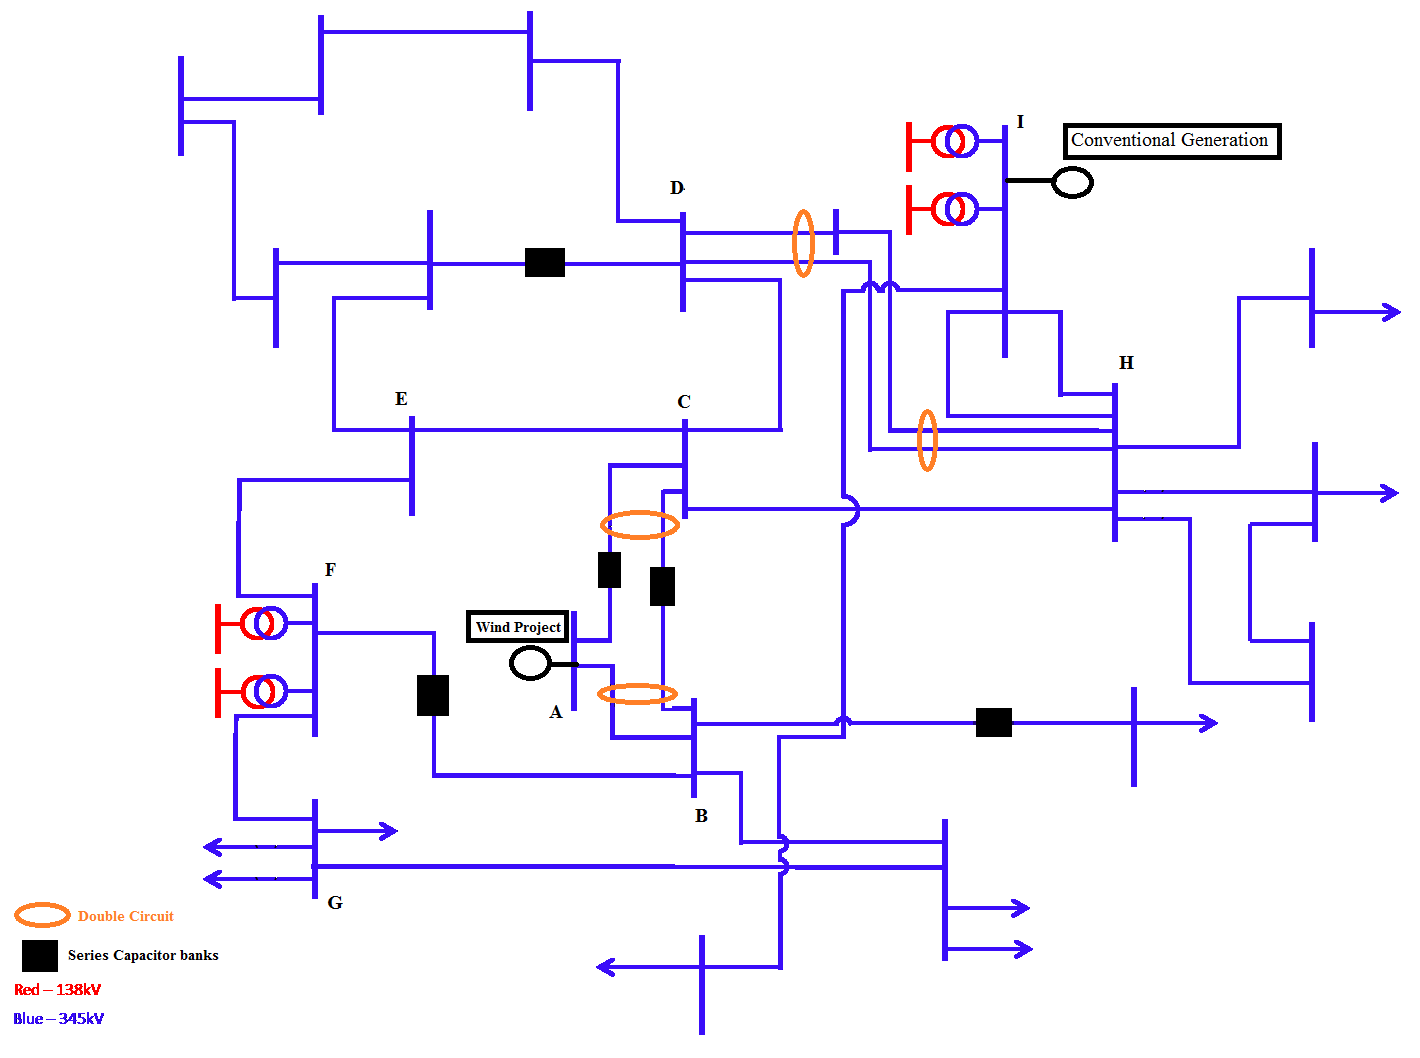
\includegraphics[scale=0.3]{artwork/SLD}\caption{Area under study\label{fig:Area-under-study}}
\end{figure}

Prior to translating the ISO system model into PSCAD\texttrademark ,
the WP was added to the PSS\textregistered E load flow case in order
to complete the network model. The WP was added to the PSS\textregistered E
case as an equivalent generator with an active and reactive power
capability according to the project specifications. The PSS\textregistered E
model was prepared for translation by running a load flow study including
the WP to control the voltage at the POI. The authors then selected
the buses shown in \figref{Area-under-study} within the PSS\textregistered E
power flow case for direct inclusion in the PSCAD\texttrademark{}
case. Afterwards, we performed a frequency scan in the PSCAD\texttrademark{}
case at the POI of the project. The authors then added new buses from
all directions around the WP until the frequency scan did not change
in an appreciable manner from one scan to another as a result of the
addition of the new buses. After selecting the buses that will be
retained in the PSCAD\texttrademark{} case, the remainder of ISO system
model was modeled as equivalent voltage sources behind impedances
such that the power flow is preserved in the PSCAD\texttrademark{}
case as in the PSS\textregistered E case. It should be noted that
no generators other than WP were modeled in detail for this study;
any generator translated into PSCAD\texttrademark{} was modeled as
an ideal voltage source behind an impedance.

Additionally, we modeled all of the series capacitor banks in \figref{Area-under-study}
with a proprietary protection model provided by the TSO. The model
has been set up according with the settings provided by TSO. It should
be noted that all the series capacitor banks shown in \figref{Area-under-study}
are always 24 \textgreek{W} per the information provided by the TSO.
It should be noted that the series capacitors are compensation more
than 100\% of the line length in all cases. 

A detailed model of WP was developed in PSCAD\texttrademark . The
detailed model contains all project equipment up to the high side
of the project main power transformer. Additionally, this model includes
the ability to activate and deactivate the feeder circuit breakers,
shunt reactive devices, and the series compensation firmware. The
transmission tie line was added to the output of the detailed model
to complete the WP. The WP was assumed to operate under normal configuration
with all feeder breakers, shunt reactive devices and the series compensation
option all turned ON. 

Surge arresters were added at the POI of the project at bus A. It
should be noted that all series capacitors in the ISO case are installed
at the midpoint of the respective transmission lines. 

Lastly, the WP detailed model was inserted into the ISO PSCAD\texttrademark{}
equivalent model, described above at the POI at Bus A as shown in
\figref{Area-under-study}, replacing the equivalent representation
of the project created for the PSS\textregistered E load flow case.
It should be noted that the wind turbines come with a proprietary
software that can introduce synthetic inertia to the rotor in case
SSO is detected. This has been modeled as well. 

\section{Frequency Scan Screening Study\label{sec:Frequency-Scan-Screening}}

A frequency scan screening study has been performed according to \cite{el1983use}.
The feedback effect of the grid on the turbine impedance as given
in \cite{renfreqscan} has not been taken into consideration to produce
conservative results. The grid frequency scan is described in \subsecref{Grid-Side-Frequency}
while the project side frequency scan is provided in \subsecref{Project-Side-Frequency}.
The combined grid and project frequency scan is presented in \subsecref{Combined-Frequency-Scan}. 

\subsection{Grid Side Frequency Scan \label{subsec:Grid-Side-Frequency}}

A grid side frequency scan was performed to determine the contingencies,
if any, up to N-5 that result in the WP to become near radial or radially
connected to the series compensated transmission lines in \figref{Area-under-study}.
A frequency scan of the transmission system was performed for WP at
the proposed POI at bus A. The frequency scan was used to calculate
the equivalent resistance and reactance looking into the transmission
network at the project\textquoteright s POI for different contingency
conditions, up to N-5, that may show vulnerability to SSO due to becoming
radially connected to series compensation capacitors. 

Additionally, for each of these contingencies, we evaluated various
combinations of sensitivities. These sensitivities pertain to whether
the turbine series compensation option is turned ON or OFF, whether
the switched shunts provided in \tabref{Switched-Shunts-Sensitivities}
are switched ON or OFF and whether the series capacitor banks in \figref{Area-under-study}
are ON or OFF. 
\begin{table}[h]
\caption{Switched Shunts Sensitivities\label{tab:Switched-Shunts-Sensitivities}}

\begin{centering}
\begin{tabular}{cccc}
\toprule 
Location & Type & \# of steps and MVAr size & Configuration\tabularnewline
\midrule 
Bus D & Reactor & 4-50 & ON/OFF\tabularnewline
\midrule 
Bus D & Capacitor & 2-130.9 & ON/OFF\tabularnewline
\midrule 
Bus C & Reactor & 4-50 & ON/OFF\tabularnewline
\midrule 
Bus C & Capacitor & 2-130.9 & ON/OFF\tabularnewline
\midrule 
Bus B & Reactor & 6-50 & ON/OFF\tabularnewline
\midrule 
Bus G & Capacitor & 2-80 & ON/OFF\tabularnewline
\midrule 
Bus H & Reactor & 3-50 & ON/OFF\tabularnewline
\midrule 
Bus E & Reactor & 3-50 & ON/OFF\tabularnewline
\midrule 
Bus E & Capacitor & 2-50 & ON/OFF\tabularnewline
\bottomrule
\end{tabular}
\par\end{centering}
\end{table}

The sensitivity analysis with regards to the switched shunts provided
in \tabref{Switched-Shunts-Sensitivities} has revealed that the status
of those switched shunts has minimal effect on the grid side frequency
scan. During the sensitivity analysis with regards to the switched
shunts, we elected to switch all shunts ON or OFF at once to observe
the effect on the grid side frequency scans in order to determine
a worst case scenario. Switching all shunts ON or OFF at once does
not cause appreciable difference in the grid frequency scan for all
contingencies considered. Thus, for all subsequent analysis, the switched
shunts given in \tabref{Switched-Shunts-Sensitivities} has been either
turned ON or OFF completely for the purpose of studying other sensitivities.

It is important to note that for each contingency case considered,
the power flow case was convergent and solved for high and low wind
conditions. The grid side frequency scan in the base case with no
contingencies is given in \figref{Grid-side-frequency}. Note that
the grid frequency scan is the same for both the cases when all switched
shunts are OFF or ON. The grid side frequency scan for all contingency
cases are shown in \figref{Grid-side-frequency-1}. It is to be noted
that the grid has relatively small impedance even under the base case
with no contingencies 
\begin{figure}[h]
\begin{centering}
\includegraphics[scale=0.4]{\string"artwork/base Freq scan\string".eps}\caption{Grid side frequency scan with no contingencies (Impedance is in per
unit of system base)\label{fig:Grid-side-frequency}}
\par\end{centering}
\end{figure}
\begin{figure}[h]
\begin{centering}
\includegraphics[scale=0.3]{artwork/sysReport}\caption{Grid side frequency scan for all contingencies considered along with
their sensitivities \label{fig:Grid-side-frequency-1}}
\par\end{centering}
\end{figure}

The results of the system side frequency scan indicate that the reactance
of the system can become negative for all contingency conditions up
to and including N-5 contingencies for all sensitivities considered.
However, for all contingency conditions up to and including N-5 contingencies,
the system resistance is positive, albeit small. 

\subsection{Project Side Frequency Scan \label{subsec:Project-Side-Frequency}}

A project side frequency scan of the WP was performed with and without
the series compensation firmware to determine the total net impedance
of the WP given its specifications. This frequency scan looked into
the wind project from the POI and included the wind turbines, the
most recent collection system design and layout as well as the current
main power transformer and pad mount transformer specifications.

The purpose of this study is to observe the impedance of the wind
project over the range of frequencies under consideration to determine
if the wind project provides a positive resistance at the POI to dampen
out any resonance created from system disturbances.

The results from the project frequency scan shows that the reactance
of the project is positive for all frequencies under study. The project
frequency scans are shown in \figref{Project-side-frequency_10_seriesOFF},
\figref{Project-side-frequency_100_seriesOFF}, \figref{Project-side-frequency_10_seriesON}and
\figref{Project-side-frequency_100_seriesON}for 10\% and 100\% output,
respectively with and without the series compensation software. The
series compensation firmware being engaged shows a benefit in shifting
the low resistance point of the wind turbine to be further away from
the typical SSO resonance point and therefore was recommended to be
engaged for the liftetime of the project. 
\begin{figure}[h]
\begin{centering}
\includegraphics[scale=0.6]{\string"artwork/frequency scan for 10% turbine output with series compensation option\string".eps}\caption{Project side frequency scan for 10\% turbine output without series
compensation option\label{fig:Project-side-frequency_10_seriesOFF}}
\par\end{centering}
\end{figure}
\begin{figure}[h]
\begin{centering}
\includegraphics[scale=0.6]{\string"artwork/for 100% turbine output without series compensation option\string".eps}\caption{Project side frequency scan for 100\% turbine output without series
compensation option\label{fig:Project-side-frequency_100_seriesOFF}}
\par\end{centering}
\end{figure}
\begin{figure}[h]
\begin{centering}
\includegraphics[scale=0.6]{\string"artwork/frequency scan for 10% turbine output with series compensation option\string".eps}
\par\end{centering}
\caption{Project side frequency scan for 10\% turbine output with series compensation
option\label{fig:Project-side-frequency_10_seriesON}}

\end{figure}
\begin{figure}[h]

\begin{centering}
\includegraphics[scale=0.6]{\string"artwork/for 100% turbine output with series compensation option\string".eps}\caption{Project side frequency scan for 100\% turbine output with series compensation
option\label{fig:Project-side-frequency_100_seriesON}}
\par\end{centering}
\end{figure}
\begin{figure}[h]
\centering{}\includegraphics[width=0.4\textwidth,height=0.3\paperheight]{artwork/ssrStudy_On_10}\caption{Combined gird and project frequency scan (10\% output in the top and
100\% in the lower graph)\label{fig:Combined-gird-and}}
\end{figure}


\subsection{Combined Frequency Scan \label{subsec:Combined-Frequency-Scan}}

The system frequency scans given in \figref{Grid-side-frequency-1}
and the project frequency scans shown previously \subsecref{Project-Side-Frequency}
are combined in \figref{Combined-gird-and} for both the 10\% and
100\% project output. 

The combined grid and project scans show that the combined reactance
can become below zero from 0 Hz to 12 Hz of the frequency range under
consideration for both the 10\% and 100\% dispatch levels with and
without the series compensation firmware engaged for all contingency
conditions along with the sensitivities considered. For the 10\% percent
dispatch level, the combined resistance can become negative from 33
Hz to 44 Hz in case the series compensation option is engaged and
25 Hz to 34 Hz in case the compensation option is not engaged for
the majority of the contingencies and sensitivities considered. Thus
the combined resistance is never negative when the combined reactance
crosses zero. 

We concluded that the WP is unlikely to be susceptible to SSO for
all cases considered even when the wind project is not equipped with
the series compensation firmware. 

A detailed EMT study was then performed in \secref{Detailed-EMT-Study}
to fully assess the susceptibility of WP for SSO for the N-1 contingency
conditions and corresponding sensitivities. This is done to provide
a firm answer on whether the negative resistance in case of the 10\%
dispatch level can cause SSO and to answer whether the resistance
is high enough to damp any SSO in case the 100\% dispatch level.

\section{Detailed EMT Study\label{sec:Detailed-EMT-Study}}

The system model was set up according to what has been mentioned in
\secref{System-Model}. After that, we modified the PSCAD\texttrademark{}
case manually by introducing a fault logic to the line A-B. The outage
of this line causes the project to be radially connected to the series
capacitor banks installed on the line A-C. The fault logic would create
a bolted three phase to ground fault on the midpoint of the line A-B
and clear the fault by opening the circuit breakers at both line ends
after five (5) cycles. 

After that, the fault logic would be activated after the PSCAD\texttrademark{}
case reaches steady state. In all of the cases in this study, it was
found that the PSCAD\texttrademark{} cases reach steady state at 1.3
seconds. The fault logic is then invoked at 1.3 seconds by creating
the bolted three phase to ground fault on the midpoint of line A-B
and then clearing the fault in five (5) cycles (t = 1.383 seconds).
The active power, reactive power, three phase voltage, RMS voltage,
trip code of the turbines within the WP as well as three phase currents
at the POI of the project were all monitored for 10 seconds. 

Analysis revealed that the WP will trip offline following clearing
of the fault on the line A-B for all of the scenarios considered.
In some cases, the project would trip due to overcurrent while in
other cases the trip was due to overvoltage. The current output of
the project, MW and MVAr as well as the POI voltage are shown in \figref{Output-current-of},
\figref{Active-and-reactive} and \figref{Voltage-at-POI}, respectively.
\begin{figure}[h]
\begin{centering}
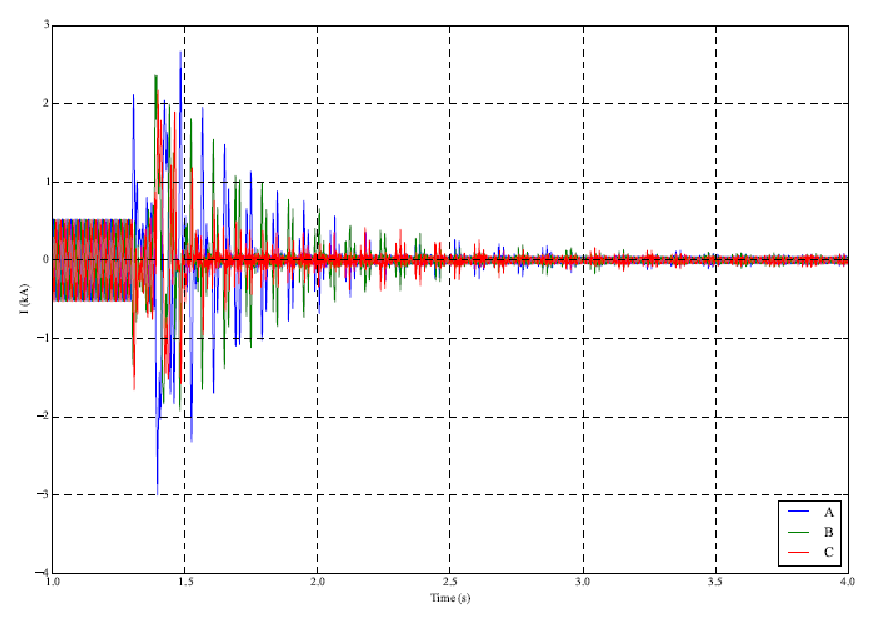
\includegraphics[scale=0.6]{artwork/currents}
\par\end{centering}
\caption{Output current of the WP\label{fig:Output-current-of}}

\end{figure}
\begin{figure}[h]
\begin{centering}
\includegraphics[scale=0.6]{\string"artwork/MW and MVAr\string".eps}\caption{Active and reactive power output of the WP\label{fig:Active-and-reactive}}
\par\end{centering}
\end{figure}
\begin{figure}[h]

\begin{centering}
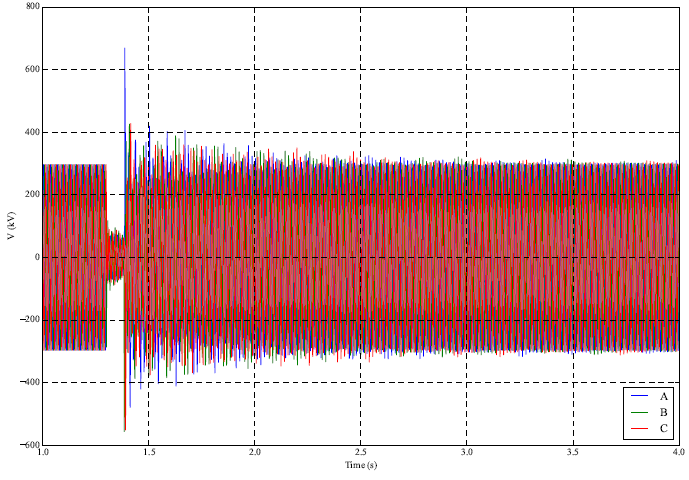
\includegraphics[scale=0.6]{artwork/voltage}\caption{Voltage at POI \label{fig:Voltage-at-POI}}
\par\end{centering}
\end{figure}


\section{Investigation of the trip after clearing the fault\label{sec:Investigation-of-the-trip}}

As can be seen from \figref{Active-and-reactive}, following the clearing
of the fault the project absorbs high amount of reactive power. Additionally
as evident from \figref{Voltage-at-POI}, the instantaneous voltage
at the POI is beyond the high voltage ride through capability of any
ISO. It is to be noted that the surge arrester at the POI is not able
to clip the voltage to acceptable values due to the unusually high
amount of reactive power that is absorbed by the project. 

Root cause analysis has shown that the reactive power is being pushed
from the series capacitor banks to the project after clearing the
fault. The TSO has designed the protection of all of the series capacitor
banks in the system such that they ride through the most severe fault.
A fault in line A-B is not an exception to this. This is mainly done
for stability enhancement and increasing the power transfer capability
in the region under certain loading and generation scenarios. 

The problem can be understood by referring to \figref{Fault-and-clearing}.
In this figure, it can be seen that once the fault occurs on line
A-B, the voltage across the capacitor banks become close to full line
to line voltage of 345 kV and the capacitor bank store a massive amount
of reactive power as a result. However, once the fault is cleared
by opening the circuit breakers at both ends of the line A-B, the
voltage across the capacitor bank returns to normal which is around
27 kV. Since the voltage across the capacitor cannot change instantaneously,
the capacitor bank releases the previously stored energy back to the
system in both directions and the voltage across the capacitor bank
starts to overshoot. Since the WP is radially connected and very close
electrically to the series capacitor banks, it attracts most of the
reactive power. The reactive power absorbed greatly exceeds capability
of the the turbines and they trip offline as a result. 
\begin{figure}[h]
\begin{centering}
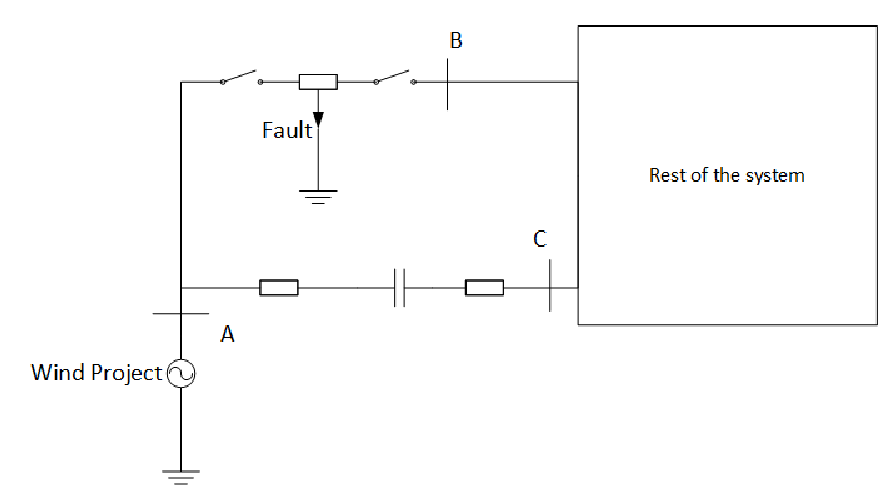
\includegraphics[scale=0.6]{artwork/cap}\caption{Clearing the fault on line A-B\label{fig:Fault-and-clearing}}
\par\end{centering}
\end{figure}


\section{Conclusions \label{sec:Conclusions}}

An study has been performed to assess whether the WP under construction
will be susceptible to SSO. A frequency scan screening study was performed
and indicated that the WP is unlikely to suffer SSO even though is
right next door to a large series compensation device. A detailed
EMT study was performed to to confirm the findings of the frequency
scan screening study. EMT simulations showed that the project will
trip after clearing the fault on one line the outage of which will
cause the project to be radially connected to the series compensation
capacitor. Investigations were carried out to understand the nature
of this trip. The authors concluded that the trip is due to the high
voltage and reactive power surge coming back from the series capacitors
after the fault is cleared. The project was thus not susceptible to
SSO. The ISO was notified of the findings and approved the study. 

\section*{Acknowledgment }

The authors would like to thank Dustin Howard and Nath Venkit of GE
for their help and support throughout the study. 

\bibliographystyle{IEEEtran}
\bibliography{refs}

\end{document}
